% !TeX root = ../main.tex
% Scene thumbnails are independent author examples, not a cross-method experiment.
%
% Design (2026-10-28): the three routes are laid out on ONE shared column grid so
% that the figure argues a comparison instead of listing three rows. The columns
% are: example / route / input / PREDICTION / output. The prediction column is
% the axis of comparison:
%   - VLA leaves it empty          -> the action is produced without explicitly
%     predicting the consequence;
%   - prediction-assisted operation fills it -> the consequence is predicted and
%     then used to choose among candidate actions;
%   - WAM spans it together with the output -> future observation and action are
%     generated jointly.
% Input and output slots are white, the prediction slot is tinted, and the
% separators stop short of the margins so the block still reads as one figure.
\begingroup
\linespread{1}\selectfont
\begin{tikzpicture}[
  x=1cm,y=1cm,text=black,line cap=round,line join=round,
  font=\songti\fontsize{9.6pt}{12pt}\selectfont,
  every node/.style={align=center,outer sep=0pt,inner sep=0pt},
  laHead/.style={font=\heiti\fontsize{9.6pt}{12pt}\selectfont},
  laRoute/.style={font=\heiti\fontsize{10pt}{12.5pt}\selectfont},
  laSource/.style={font=\fontsize{8.5pt}{10.5pt}\selectfont,text=black!62},
  laSlot/.style={draw=black,line width=0.6pt,fill=white,
    minimum height=0.92cm,inner xsep=6pt},
  laPred/.style={laSlot,fill=black!9},
  laArrow/.style={draw=black,line width=0.7pt,
    -{Latex[length=1.6mm,width=1.1mm]}}
]
  \path[use as bounding box] (0,0.30) rectangle (16,6.66);

  % ---------- shared column grid ----------
  \def\cIn{7.05}    % input slot centre
  \def\cPred{10.30} % prediction slot centre
  \def\cOut{13.65}  % output slot centre
  \def\rowSep{0.20} % separators start here, leaving a margin on both sides
  \def\rowSepEnd{15.80}

  % ---------- header ----------
  \node[laHead,anchor=west] at (0.28,6.38) {场景示例};
  \node[laHead] at (4.20,6.38) {研究路线};
  \node[laHead] at (\cIn,6.38) {输入};
  \node[laHead] at (\cPred,6.38) {是否预测后果};
  \node[laHead] at (\cOut,6.38) {输出};
  \draw[black!40,line width=0.5pt] (\rowSep,6.14) -- (\rowSepEnd,6.14);

  % ---------- row 1: VLA ----------
  \node at (1.60,5.30)
    {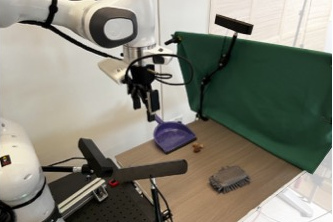
\includegraphics[height=1.10cm]{figures/generated/literature_review/openvla_scene.jpg}};
  \node[laSource] at (1.60,4.56) {OpenVLA};
  \node[laRoute] at (4.20,4.98) {VLA};
  \node[laSlot,minimum width=2.35cm] at (\cIn,4.98) {观测＋任务};
  % the arrow crosses the empty prediction column on purpose
  \draw[laArrow] (8.32,4.98) -- (12.28,4.98);
  \node[laSource,fill=white,inner xsep=3pt] at (\cPred,4.98) {不经预测};
  \node[laSlot,minimum width=2.55cm] at (\cOut,4.98) {动作};

  \draw[black!20,line width=0.4pt] (\rowSep,4.16) -- (\rowSepEnd,4.16);

  % ---------- row 2: prediction-assisted operation ----------
  \node at (1.60,3.40)
    {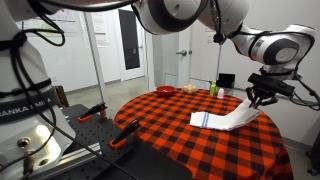
\includegraphics[height=1.10cm]{figures/generated/literature_review/point_observation_v1.jpg}};
  \node[laSource] at (1.60,2.66) {PointWorld};
  \node[laRoute] at (4.20,3.08) {预测辅助\\操作};
  \node[laSlot,minimum width=2.35cm] at (\cIn,3.08) {状态＋\\候选动作};
  \draw[laArrow] (8.32,3.08) -- (9.30,3.08);
  \node[laPred,minimum width=1.90cm] at (\cPred,3.08) {预测后果};
  \draw[laArrow] (11.34,3.08) -- (12.28,3.08);
  \node[laSlot,minimum width=2.55cm] at (\cOut,3.08) {动作选择};

  \draw[black!20,line width=0.4pt] (\rowSep,2.26) -- (\rowSepEnd,2.26);

  % ---------- row 3: world action model ----------
  \node at (1.60,1.50)
    {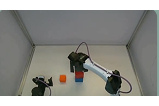
\includegraphics[height=1.10cm]{figures/generated/literature_review/dreamzero_scene.jpg}};
  \node[laSource] at (1.60,0.76) {DreamZero};
  \node[laRoute] at (4.20,1.18) {WAM};
  \node[laSlot,minimum width=2.35cm] at (\cIn,1.18) {观测＋任务};
  \draw[laArrow] (8.32,1.18) -- (9.30,1.18);
  % one slot spanning prediction and output: the two are generated together
  \node[laPred,minimum width=5.85cm] at ({(9.30+15.15)/2},1.18)
    {未来视频＋动作\quad{\fontsize{8.5pt}{10.5pt}\selectfont（联合生成）}};
\end{tikzpicture}
\endgroup
